\section{Encode Experiments} \label{integr-encode-exper-sect}
To evaluate the performance of the BCC model, we will use the same ENCODE datasets that were described in \emph{Section \ref{encode-data-sect}}, that is, the RRBS and RNA-Seq data produced from K562 and H1-hESC cell lines.

\subsection{Data Processing}
The procedure for preprocessing the raw experimental data and defining promoter regions is exactly the same as described in \emph{Section \ref{meth-encode-experiments-sect}}. 

To perform integrative clustering we have to define the data sources $m$ and the observation models $f_{m}(X_{mn}|\theta_{m})$ that each data source follows. 
For our experiments we have two data sources: (1) RNA-Seq which measure gene expression (GE) and (2) RRBS which measure CpG methylation (ME). Each source is available for a common set of N objects, where each object is a protein-coding gene.

RNA-Seq experiments return count based measure of gene expression and a natural choice to statistically model these data is a \emph{Poisson} observation model. Thus, we assume that each object from the RNA-Seq data source is generated from a Poisson mixture distribution:
\begin{equation}
	X_{mn} \mid L_{mn} = k, \theta_{mk} \sim \mathcal{P}ois\big(\lambda_{mk}\big)
\end{equation}

The measurement process of DNA methylation from RRBS experiments can be modelled with a Binomial distribution. Since our objects are protein-coding genes it does not make sense to model each CpG site, but rather we should consider promoter regions and model the methylation level of these regions. A promising approach would be to model each methylation profile using the \emph{Binomial distributed Probit regression} model introduced in \emph{Chapter \ref{model-meth-chapter}}. Even though this model is promising, it cannot be directly integrated in the BCC model, as we will explain in \emph{Section \ref{conc-meth-prof-bcc-subsect}}.

Hence, in order to evaluate the RRBS data with the BCC model, we take a crude approach by summing the methylation level of all the CpGs in each promoter region. Assuming \emph{independence} of the methylation level between CpG sites, the sum of independent Binomial random variables will also follow a Binomial distribution. Thus, we assume that each object from the RRBS data source is generated from a Binomial mixture distribution:
\begin{equation}
	X_{mn} \mid L_{mn} = k, \theta_{mk} \sim \mathcal{B}inom\big(t_{mk}, \rho_{mk}\big)
\end{equation}
where $t_{mk}$ is the sum of total number of reads for each CpG site for a specific region.

The independence assumption is a strong assumption, since the the methylation level of a CpG site is highly correlated with the methylation level of the surrounding CpGs (i.e. spatial co-dependence). Also, by summing the methylation level of the CpGs in each region and representing each promoter with a single methylation value, essentially we discard  important features of the data. For example, methylation profiles with low methylation upstream of TSS and high methylation downstream of TSS, would have similar methylation value with their reverse pattern, that is, methylation profiles with high methylation upstream of TSS and low methylation downstream of TSS. These issues, need to be understood and taken into consideration when analysing the results of the BCC model.

\subsection{Method evaluation} \label{integr-method-eval-subsect}
To evaluate the performance of the BCC model on these real datasets, we decided to concatenate the different experiments conducted on each cell line, resulting in 2-dimensional datasets for each data source. That is, for the RRBS data source, the $1^{st}$ dimension will be the experiments for the K562 cell line and in the $2^{nd}$ dimension the ones for the H1-hESC cell line. Similarly for the RNA-Seq data source.

After pre-processing each dataset individually, we mapped the TSS of the genes from both datasets. This procedure resulted in 604 protein-coding genes for testing. The total number of MCMC iterations was set to $T=20,000$ and the first $5,000$ iterations were discarded, \ie burn-in period. The total number of clusters K was set to 3. This was an empirical choice, since a bigger number would result in empty clusters or clusters with only a few objects assigned to them. 

\emph{Fig. \ref{bcc2D-pic}} provides scatter plots of the datasets for the RRBS source (ME) and the RNA-Seq source (GE). For each object the source-specific and overall cluster index is shown, together with the adherence parameter $\alpha$. Each point depicts a 2-dimensional object, where the \emph{x-axis} denotes the K562 cell line and the \emph{y-axis} the H1-hESC cell line. Each object is coloured according the overall clustering assignment; cluster 1 is black, cluster 2 is red and cluster 3 is blue. Symbols indicate source-specific cluster assignments; cluster 1 is represented with filled circles ($\bullet$), cluster 2 with plus signs (+) and cluster 3 with asterisks ($\ast$). 

We observe that the ME source has higher adherence to the overall clustering, $\alpha=0.89$, whereas the GE source has only $\alpha=0.48$. We argue that this behaviour may be related with the fact that the majority of ME object are unmethylated, and the algorithm tries to explain better these densely concentrated samples in order to increase its accuracy with the expense of having a lower adherence for the GE source, whose objects are more spread out.

The source-specific clusters have a clear biological interpretation, for the ME data source we have unmethylated, medium-methylated and hyper-methylated clusters of promoter regions, and similarly for the GE data source we have clusters according to different gene expression levels. It is also clear that the promoters of the K562 cell line are highly methylated compared to the H1-hESC cell line, which could be related to the fact that the K562 cells are \emph{cancer} cells. 

In general, the source-specific clusterings (\ie symbols) are well distinguished, in contrast to the overall clusterings (\ie colours). However, the overall clusterings are also evident for both data sources and to some degree show the clear association between promoter methylation and gene expression. We observe that highly methylated promoters (\emph{red colour}) result in silencing gene expression. On the other hand, unmethylated promoters (\emph{black colour}) in general are associated with high transcriptional activity \citep{Deaton2011}. These findings confirm the results shown in \emph{Section \ref{meth-encode-experiments-sect}} and also numerous studies that relate promoter methylation patterns with regulation of gene expression. 
\begin{figure}[ht!]
     \begin{center}
        \subfigure[]{
            \label{bccME2D:first}
            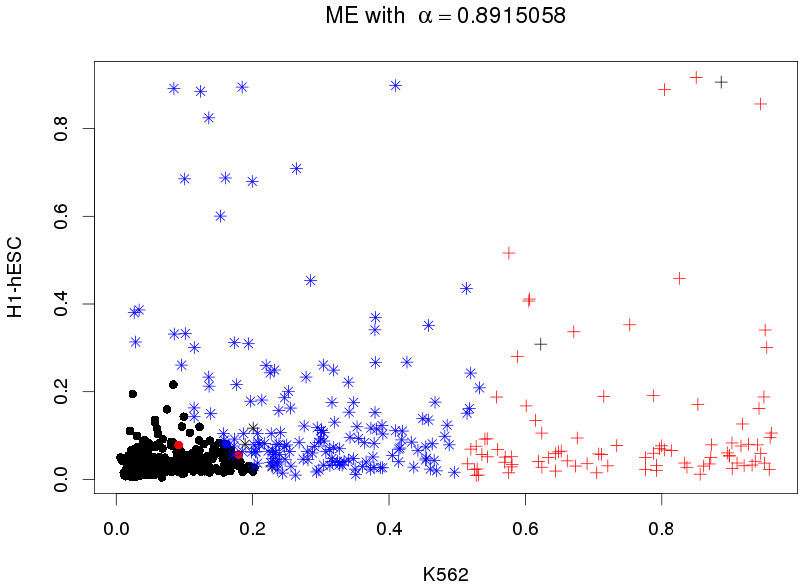
\includegraphics[width=0.48\textwidth]{images/bccME2D-2}
        }
        \subfigure[]{
           \label{bccGE2D:second}
           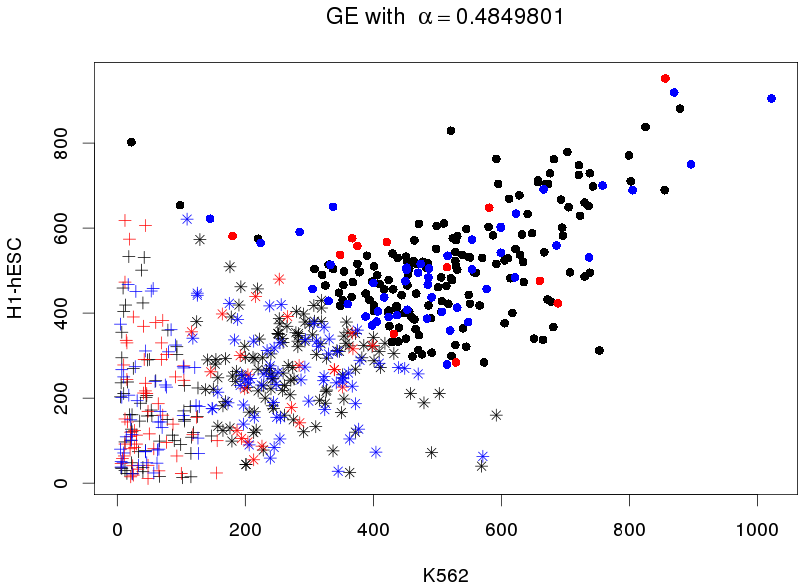
\includegraphics[width=0.48\textwidth]{images/bccGE2D-2}
        }
    \end{center}
    \caption{\emph{Scatter plots for each data source; (a) RRBS source and (b) RNA-Seq source. The \emph{x-axis} denotes the K562 cell line, and the \emph{y-axis} denotes the H1-hESC cell line. Each object is coloured according the overall clustering assignment; cluster 1 is black, cluster 2 is red and cluster 3 is blue. Symbols indicate source-specific cluster assignments; cluster 1 is represented with filled circles ($\bullet$), cluster 2 with plus signs (+) and cluster 3 with asterisks ($\ast$).}}
   \label{bcc2D-pic}
\end{figure}

Further technical details for performing this experiment are given in \emph{Appendix \ref{app-mcmc-mixing-chapter}}. These include analysis for the mixing and convergence of the MCMC simulations to the target distribution and also provide the expected values of all the inferred model parameters.

\subsection*{Combining technical replicates}
Motivated by these results, we decided to perform further experiments with the K562 and H1-hESC cell lines. In most cases when designing biological experiments, technical replicates are also performed to validate the results. For the ENCODE datasets we have:
\begin{itemize}
	\item \emph{RRBS experiments}: two replicates for the K562 cell line and two replicates for the H1-hESC cell line.
	\item \emph{RNA-Seq experiments}: two replicates for the K562 cell line and four replicates for the H1-hESC cell line.
\end{itemize}

Hence, by concatenating both cell lines and their replicates for each data source would result in a 4-dimensional ME data source and a 6-dimensional GE data source.  After pre-processing each dataset and mapping the TSS of the genes from all datasets, we were left with 554 protein-coding genes for testing. We run the BCC model for $T=20,000$ iterations, the first $5,000$ iterations were discarded for the burn-in period, and we selected K=3 clusters. 

\emph{Fig. \ref{bccMV-pic}} provides scatter plots of the first two principal components for the RRBS source (ME) and the RNA-Seq source (GE). Similarly to \emph{Fig. \ref{bcc2D-pic}} for each sample the source-specific and the overall cluster index are shown, together with the adherence parameter $\alpha$. The ME source has still higher adherence to the overall clustering with $a=0.87$, whereas the GE has $a=0.50$. 

In the direction of the first two principal components, the source-specific clusterings again are well distinguished from each other, however the overall clusterings are more difficult to interpret; especially for the GE data source. For brevity, analysis for the mixing of the MCMC chains for each parameter is not shown in this document, but the chains in general were mixing quite well, similarly to the ones shown in \emph{Appendix \ref{app-mcmc-mixing-chapter}} for the previous experiments.
\begin{figure}[ht!]
     \begin{center}
        \subfigure[]{
            \label{bccMEMV:first}
            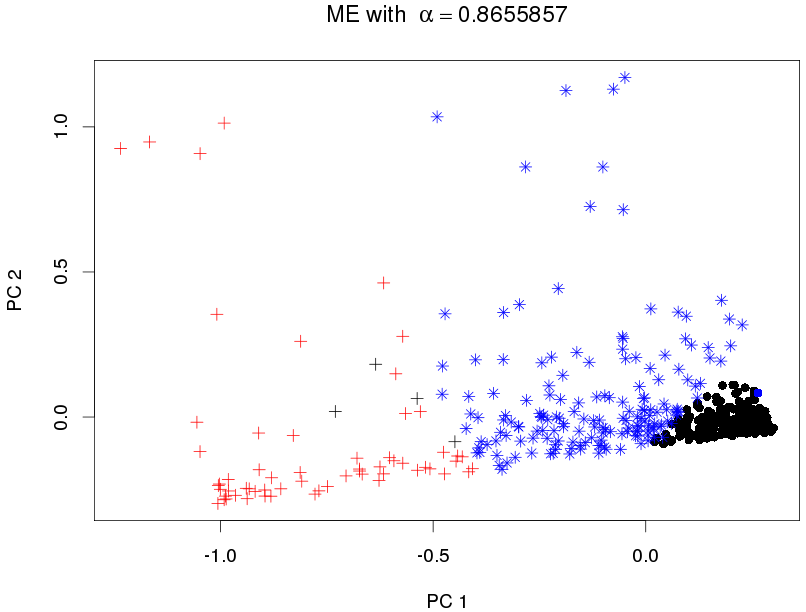
\includegraphics[width=0.48\textwidth]{images/bccMEMV-2}
        }
        \subfigure[]{
           \label{bccGEMV:second}
           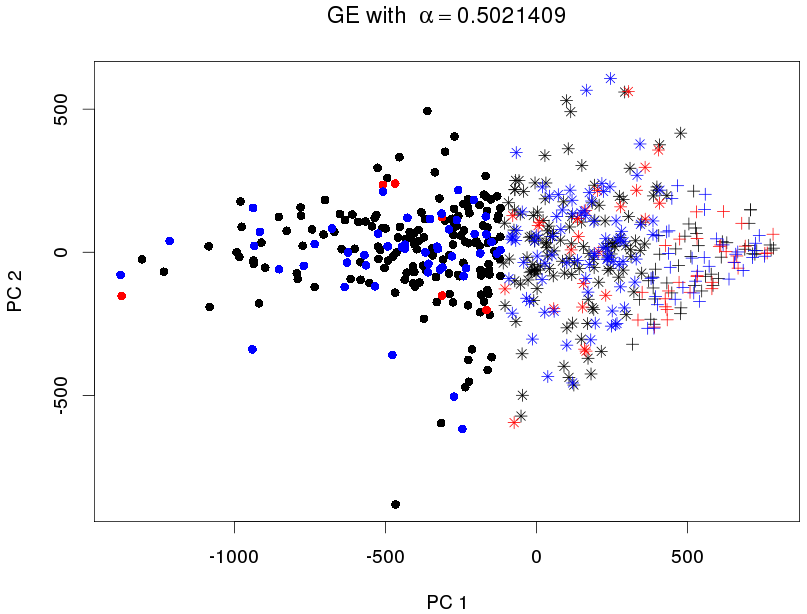
\includegraphics[width=0.48\textwidth]{images/bccGEMV-2}
        }
    \end{center}
    \caption{\emph{Scatter plots of the first two principal components for each data source; (a) RRBS source and (b) RNA-Seq source. Each object is coloured according the overall clustering assignment; cluster 1 is black, cluster 2 is red and cluster 3 is blue. Symbols indicate source-specific cluster assignments; cluster 1 is represented with filled circles ($\bullet$), cluster 2 with plus signs (+) and cluster 3 with asterisks ($\ast$). See the text for details.}}
   \label{bccMV-pic}
\end{figure}